% =============================================================================
% COPYRIGHT AND DISCLAIMER
% =============================================================================
% This file is provided as a convenience template for competition participants.
% By using it, you accept full responsibility for compliance with all applicable
% copyright, licensing, and usage rules of the Association for Computing
% Machinery (ACM) and of any LaTeX packages you load (including, without
% limitation, the "acmart" document class and related ACM materials).
%
% Consult ACM's official publication, template, and copyright policies before
% using this setup for any purpose other than this competition. Do not assume
% that this template may be reused, redistributed, or submitted elsewhere
% without independently verifying ACM's current rules.
%
% Use of the "acmart" class, the "sigconf" option, or ACM-style formatting in
% this template does NOT mean that this report, this competition, its organizers,
% or any resulting PDF is sponsored, endorsed, affiliated with, or published by
% ACM. ACM trademarks and branding remain the property of ACM.
%
% Template packages live in preamble.tex.
% Citations live in main.bib. Edit this file with your paper content.
% =============================================================================
% Built from the organizers' Overleaf template (https://www.overleaf.com/read/vjztpvrnbrdh),
% downloaded 2026-10-24; the untouched originals are in template_original/.
% Our citations are in references.bib (main.bib keeps the organizers' two entries).
% Every number in this file is traced in NUMBERS.md.

\documentclass[sigconf]{acmart}
% =============================================================================
% Template setup — participants normally do not edit this file.
% Author content belongs in main.tex; citations belong in main.bib.
% \documentclass lives in main.tex so Overleaf does not treat this file as root.
% =============================================================================

% --- Competition / non-ACM-submission friendly rights metadata -------------
\setcopyright{none}
\settopmatter{printacmref=false}
\acmConference[Kaggle Competition]{Filament Segmentation Challenge}{2026}{\href{https://www.kaggle.com/competitions/filament-segmentation-2026}{kaggle.com/competitions/filament-segmentation-2026}}
\acmBooktitle{Competition Report}
\acmDOI{}
\acmISBN{}

% --- Author guidance text --------------------------------------------------
% \guide{...} is gray italic while \guideStyletrue; omitted from the PDF if false.
% Flip the switch in main.tex after % =============================================================================
% Template setup — participants normally do not edit this file.
% Author content belongs in main.tex; citations belong in main.bib.
% \documentclass lives in main.tex so Overleaf does not treat this file as root.
% =============================================================================

% --- Competition / non-ACM-submission friendly rights metadata -------------
\setcopyright{none}
\settopmatter{printacmref=false}
\acmConference[Kaggle Competition]{Filament Segmentation Challenge}{2026}{\href{https://www.kaggle.com/competitions/filament-segmentation-2026}{kaggle.com/competitions/filament-segmentation-2026}}
\acmBooktitle{Competition Report}
\acmDOI{}
\acmISBN{}

% --- Author guidance text --------------------------------------------------
% \guide{...} is gray italic while \guideStyletrue; omitted from the PDF if false.
% Flip the switch in main.tex after % =============================================================================
% Template setup — participants normally do not edit this file.
% Author content belongs in main.tex; citations belong in main.bib.
% \documentclass lives in main.tex so Overleaf does not treat this file as root.
% =============================================================================

% --- Competition / non-ACM-submission friendly rights metadata -------------
\setcopyright{none}
\settopmatter{printacmref=false}
\acmConference[Kaggle Competition]{Filament Segmentation Challenge}{2026}{\href{https://www.kaggle.com/competitions/filament-segmentation-2026}{kaggle.com/competitions/filament-segmentation-2026}}
\acmBooktitle{Competition Report}
\acmDOI{}
\acmISBN{}

% --- Author guidance text --------------------------------------------------
% \guide{...} is gray italic while \guideStyletrue; omitted from the PDF if false.
% Flip the switch in main.tex after \input{preamble}.
%
% Do not use \guide{...} for \email{...}.
\usepackage{xcolor}
\newif\ifguideStyle
\guideStyletrue
\newcommand{\guide}[1]{%
  \ifguideStyle
    {\color{gray!65}\itshape #1}%
  \fi
}

% --- Math ------------------------------------------------------------------
% Do NOT load amssymb (or amsfonts): acmart already loads newtxmath, which
% defines the same symbols (e.g. \Bbbk) and causes a conflict on Overleaf.
% amsmath is already provided by acmart; mathtools extends it.
\usepackage{mathtools}

% --- Figures ---------------------------------------------------------------
% graphicx is already loaded by acmart
\usepackage{subcaption}

% --- Tables ----------------------------------------------------------------
% booktabs is already loaded by acmart
\usepackage{tabularx}
\usepackage{multirow}

% --- Bibliography style is set in main.tex (ACM-Reference-Format) ----------
.
%
% Do not use \guide{...} for \email{...}.
\usepackage{xcolor}
\newif\ifguideStyle
\guideStyletrue
\newcommand{\guide}[1]{%
  \ifguideStyle
    {\color{gray!65}\itshape #1}%
  \fi
}

% --- Math ------------------------------------------------------------------
% Do NOT load amssymb (or amsfonts): acmart already loads newtxmath, which
% defines the same symbols (e.g. \Bbbk) and causes a conflict on Overleaf.
% amsmath is already provided by acmart; mathtools extends it.
\usepackage{mathtools}

% --- Figures ---------------------------------------------------------------
% graphicx is already loaded by acmart
\usepackage{subcaption}

% --- Tables ----------------------------------------------------------------
% booktabs is already loaded by acmart
\usepackage{tabularx}
\usepackage{multirow}

% --- Bibliography style is set in main.tex (ACM-Reference-Format) ----------
.
%
% Do not use \guide{...} for \email{...}.
\usepackage{xcolor}
\newif\ifguideStyle
\guideStyletrue
\newcommand{\guide}[1]{%
  \ifguideStyle
    {\color{gray!65}\itshape #1}%
  \fi
}

% --- Math ------------------------------------------------------------------
% Do NOT load amssymb (or amsfonts): acmart already loads newtxmath, which
% defines the same symbols (e.g. \Bbbk) and causes a conflict on Overleaf.
% amsmath is already provided by acmart; mathtools extends it.
\usepackage{mathtools}

% --- Figures ---------------------------------------------------------------
% graphicx is already loaded by acmart
\usepackage{subcaption}

% --- Tables ----------------------------------------------------------------
% booktabs is already loaded by acmart
\usepackage{tabularx}
\usepackage{multirow}

% --- Bibliography style is set in main.tex (ACM-Reference-Format) ----------


% ---- report-local additions (kept here so preamble.tex stays as distributed) ----
\usepackage{tikz}
\usetikzlibrary{positioning,arrows.meta,fit}
\newcommand{\todo}[1]{{\color{red}\textbf{[TODO: #1]}}}   % must be empty before the final upload
\setlength{\emergencystretch}{1.5em}
\graphicspath{{figures/}{../eval/results/}{../eval/results/figures/}}
% Include a figure if it exists, otherwise draw a labelled placeholder box.
\newcommand{\maybefig}[3]{\IfFileExists{#1}{\includegraphics[width=#2]{#1}}%
  {\fbox{\parbox[c][#3][c]{#2}{\centering\color{red}\small placeholder: \texttt{\detokenize{#1}}}}}}

% Guide styling: \guideStyletrue = show gray italic hints; \guideStylefalse = omit them
% \guideStyletrue
\guideStylefalse

\begin{document}

\title{Cross-Fitted Instance Selection on a Multi-Annotator UNet with Detector Evidence}  % Replace this with your title
\subtitle{A Solution to the Solar Filament Segmentation Challenge 2026} % DO NOT CHANGE


\author{Hariohm Bhatt}
\affiliation{%
  \institution{\todo{institution, or delete line}}
  \city{\todo{city}}
  \country{\todo{country}}
}
\email{bhatthariohm2004@gmail.com}   % <- Replace with your own email

\begin{abstract}
    This report describes our solution to the Solar Filament Segmentation Challenge~2026, a Kaggle competition on automatic segmentation of solar filaments in GONG H-$\alpha$ observations. A four-fold UNet with an EfficientNetV2-S encoder, trained on soft multi-annotator targets with an auxiliary contact head, draws every mask; a four-fold YOLO11m-seg detector supplies existence evidence and a few extra candidates; and a gradient-boosted scorer, fitted out-of-fold, keeps a candidate only when its predicted contribution to panoptic quality (PQ) exceeds the break-even value. On date-grouped, cross-fitted out-of-fold (OOF) validation over all 707 training images (1154 annotator records) the final system reaches PQ 0.455 (SQ 0.682, RQ 0.668), against 0.448 for the UNet alone and an inter-annotator agreement of 0.340; the public leaderboard score is 0.40. We document the error structure by filament size, disk position and annotator support, the morphology of the predicted masks, and every post-V4 idea that failed our pre-registered acceptance rule.
\end{abstract}

\maketitle

\ifguideStyle
\noindent{\color{gray!65}\itshape
Guide mode is on.}
\par\medskip
\fi

\guide{Please limit your report to four (4) pages, excluding the Acknowledgment and References sections. Throughout this document, please follow these considerations:
\begin{itemize}
    \item Do not alter any text that is currently in black color (except for the emails under authors' name).
    \item Replace all gray text with your own.
    \item When you are done with the report, please replace \texttt{\textbackslash guideStyletrue} with \texttt{\textbackslash guideStylefalse}, to remove any gray text. Alternatively, you can remove any text wrapped in \texttt{\textbackslash guide\{\}},
    \item Be as succinct as possible, and only provide details regarding your own work. For example, there is no need to discuss what solar filaments are, or why filament segmentation matters.
    \item If you must, you can add extra sections.
\end{itemize}}


% ==================================== %
%              INTRODUCTION            %
% ==================================== %
\section{Introduction}
    This report goes over the details of our submitted solution to the Solar Filament Segmentation Challenge~2026 \cite{filament-segmentation-2026}. The challenge, launched on July~10,~2026, is organized by the Earth-Space AI Research (ESAIR) Lab\footnote{\href{https://www.esairlab.com/home}{www.esairlab.com/}}. This challenge utilizes the MAGFiLO dataset for evaluation of the segmentation algorithms \cite{ahmadzadeh2024dataset}. Each $2048{\times}2048$ GONG~\cite{harvey1996gong} image may carry one to three independent annotator records, and the score is PQ~\cite{kirillov2019panoptic} at IoU${>}0.5$, \emph{pooled} over all (image, annotator record) pairs: $\mathrm{PQ}=\sum_{\mathrm{TP}}\mathrm{IoU}/(|\mathrm{TP}|+\tfrac12|\mathrm{FP}|+\tfrac12|\mathrm{FN}|)$. The same prediction is thus scored against every record of an image, and predicted masks must be pixel-disjoint.
    Two facts shape our design. (i) Annotators disagree strongly: scoring one record against another gives PQ 0.340 (SQ 0.634, RQ 0.536) on the training set. (ii) Keeping a candidate adds $\tfrac12$ to the denominator per record whether or not it matches, so the PQ-optimal rule keeps a candidate iff its expected matched IoU, averaged over records, exceeds $\mathrm{PQ}/2$. We therefore separate \emph{drawing} masks (a dense network) from \emph{deciding} which to keep (a calibrated scorer), and we judge every change only by honest, cross-fitted validation.

% ==================================== %
%              METHODOLOGY             %
% ==================================== %
\section{Methodology}\label{sec:methodology}

\begin{figure}[t]
\centering
\begin{tikzpicture}[font=\scriptsize, node distance=2.2mm and 2.5mm,
  box/.style={draw, rounded corners=1.5pt, align=center, inner sep=2pt, minimum height=6mm, text width=#1},
  box/.default=2.15cm, ar/.style={-{Latex[length=1.6mm]}, thick}]
\node[box=1.55cm] (in) {GONG H$\alpha$\\$2048^2$ JPEG};
\node[box, right=of in] (pre) {disk fit $r{=}0.88$, limb-flattening $\to$ 3 ch: raw / flat / $r/R$};
\node[box=2.0cm, right=of pre] (unet) {4$\times$ UNet EffV2-S\\D4 TTA, tiles $1024/768$\\$\to$ $p_{\mathrm{fil}}$, $p_{\mathrm{contact}}$};
\node[box, below=of unet] (inst) {$p{\ge}0.4$, split at contact cores, fill holes, erode 1\,px $\to$ candidates};
\node[box, below=of pre] (yolo) {4$\times$ YOLO11m-seg\\1280\,px $\to$ boxes, masks, scores};
\node[box=1.55cm, below=of in] (fus) {fusion: evidence + det.-only candidates};
\node[box, below=of fus, xshift=6mm] (hgb) {HGB keep-scorer (cross-fitted) $\hat u$; keep if $\hat u\ge\tau$};
\node[box, right=of hgb, xshift=1mm] (out) {disjoint label map\\$\to$ COCO RLE CSV};
\draw[ar] (in) -- (pre); \draw[ar] (pre) -- (unet); \draw[ar] (unet) -- (inst);
\draw[ar] (pre) -- (yolo); \draw[ar] (inst.west) -- ++(-1mm,0) |- (fus.north east);
\draw[ar] (yolo) -- (fus); \draw[ar] (fus) -- (hgb); \draw[ar] (hgb) -- (out);
\end{tikzpicture}
\caption{End-to-end pipeline of the final submission (V4). All thresholds are fixed on OOF data; nothing is tuned on the leaderboard.}
\Description{Block diagram: preprocessing, UNet and detector branches, candidate extraction, fusion, scorer, export.}
\label{fig:pipeline}
\end{figure}

\begin{figure*}[t]
\centering
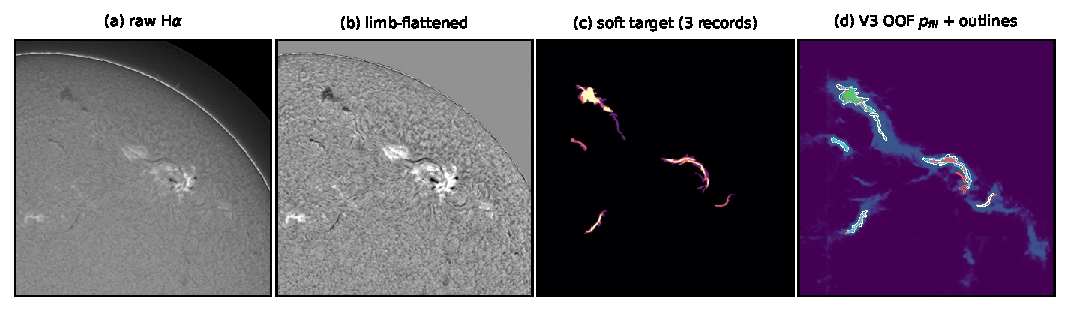
\includegraphics[width=\textwidth]{fig_data.pdf}
\caption{A training image with three annotator records (\texttt{20110306082634Lh}, $900^2$ crop, fold~1). (a) raw input; (b) limb-flattened channel; (c) soft target = mean of the three records' masks (records contain 6, 7 and 6 filaments); (d) out-of-fold V3 filament probability with each record's outlines in a different colour. The records disagree on which faint segments exist and where filaments end.}
\Description{Raw, flattened, soft-target and probability panels for one H-alpha image.}
\label{fig:data}
\end{figure*}

\textbf{Data and validation.} The training set has 707 images, 1154 annotator records and 8199 filament instances (411 images with one record, 145 with two, 151 with three; Fig.~\ref{fig:data}). We use a four-fold split grouped by observation date (folds of 177/177/177/176 images; 0 of 656 dates span two folds), frozen once and shared by every model. Each training image is predicted only by models that never saw its fold, and every second-stage model (the scorer) is itself cross-fitted over the same folds~\cite{chernozhukov2018dml}, so every reported OOF number is computed on predictions no fitted component has seen. Our PQ engine (Hungarian, IoU${>}0.5$, pooled) matches the official scorer to within 0.0002. Fold-to-fold variation is large (single-fold V3 PQ 0.424--0.452), so differences are tested pairwise: a bootstrap over images (2000 resamples, all records of an image kept together) and fold wins. \emph{Acceptance rule}, fixed before the V5 experiments: a change must gain ${\ge}0.003$ OOF PQ and win ${\ge}3$ of 4 folds.

\textbf{Preprocessing.} The solar disk is a fixed circle (radius $0.88\cdot1024$\,px). Each image is divided by its own radial limb-darkening profile (512 bins, smoothed) and then by a local median (41\,px kernel at $1/4$ resolution, ${\approx}164$ native px), giving a flattened channel; off-disk pixels are set neutral. The network sees three channels: raw intensity, flattened intensity, and normalized radius $r/R$, because filament contrast depends on disk position. No downsampling is applied: training uses native-resolution $768^2$ crops, inference $1024^2$ tiles with stride 768.

\textbf{Dense model (V3).} A UNet~\cite{ronneberger2015unet} with an ImageNet-21k EfficientNetV2-S encoder~\cite{tan2021efficientnetv2} (via \texttt{timm}/\texttt{smp}~\cite{wightman2019timm,iakubovskii2019smp}), scSE decoder attention~\cite{roy2018scse} and a full-resolution decoder stage (22.1\,M parameters) predicts two maps. The \emph{filament} target is the mean of all records' masks of the image (a soft label in $\{0,\tfrac13,\tfrac12,\dots,1\}$), so the model learns annotator consensus without sampling noise. The \emph{contact} target is the record-average of pixels where ${\ge}2$ instances, dilated by 2\,px, meet. Loss: $0.5\,\mathrm{BCE}_{\mathrm{soft}}+1.0\,\mathrm{Lov\acute{a}sz}+0.2\,\mathrm{BCE}_{\mathrm{edge}}+0.5\,\mathrm{BCE}_{\mathrm{contact}}$ (Lov\'asz hinge~\cite{berman2018lovasz}). Training: 40 epochs $\times$ 250 steps, effective batch 8, AdamW (encoder/decoder LR $3{\cdot}10^{-4}/10^{-3}$, wd 0.01, 2-epoch warm-up, cosine), bf16, EMA 0.999; crops are 50\% filament-centred and 25\% hard negatives (dark, far from any annotation); augmentation: D4, free rotation ($p{=}0.7$), scale $0.85$--$1.15$, gamma, CLAHE, blur, noise, flat-field jitter. The checkpoint is selected by PQ under a small post-processing grid on the fold's validation images. Inference averages 8 D4 views.

\textbf{Candidates.} Pixels with $p_{\mathrm{fil}}\ge0.4$ form the extent mask; connected cores with $p_{\mathrm{contact}}<0.5$ (area${\ge}16$) seed instances, and remaining extent pixels within 6\,px join the nearest core, which separates touching filaments. Holes are filled and each instance is eroded by 1\,px (all fixed on V3 OOF). Every candidate gets 12 features (area, mean/max/quantile probabilities, mean contact, elongation, major length, radius, mean raw and flattened intensity).

\textbf{Detector evidence (V4).} A YOLO11m-seg~\cite{jocher2024yolo11} per fold (1280\,px, 40 epochs, classification-loss gain 1.5, one training sample per annotator record) is run out-of-fold. Detections (score${\ge}0.05$, area${\ge}32$) add three features to the UNet candidates (best score, IoU with the detection, coverage). An unclaimed detection (score${\ge}0.10$, ${\le}30\%$ already covered) creates a new candidate drawn with UNet pixels ($p{\ge}0.2$) inside the detection grown by 4\,px. The UNet thus draws the pixels; the detector mainly votes on existence.

\textbf{Keep-scorer and export.} The regression target of a candidate is $u=\frac1R\sum_{r}\mathrm{IoU}_r\,\mathbb{1}[\mathrm{IoU}_r{>}0.5]$ over the image's $R$ records, i.e.\ its expected PQ numerator. A histogram gradient-boosting regressor~\cite{pedregosa2011sklearn} (400 iterations, LR 0.05, 31 leaves, min leaf 40, L2 1.0), weighted by $R$, is fitted on three folds and predicts the fourth; the threshold $\tau$ (0.225, near $\mathrm{PQ}/2$) is the OOF optimum (selection optimism measured at 0.0005). For the test set the scorer is refit on all OOF candidates, UNet maps are averaged over the four fold models and detections pooled over the four detectors. Because candidates are labels of one integer map, the exported masks are disjoint by construction; the CSV is audited (every RLE decodes, no empty or overlapping masks): 1077 filaments on 180 test images (5.98 per image).

% ==================================== %
%              EVALUATION              %
% ==================================== %
\section{Evaluation}\label{sec:evaluation}

\textbf{Main results and baselines.} Table~\ref{tab:main} lists our own systems and published peer systems. Peer numbers are self-reported with \emph{different} protocols and are not interchangeable with ours. V4 beats the re-scored V3 by $+0.0049$ PQ (95\% CI $+0.0022$ to $+0.0075$, 4/4 folds), mostly through precision (0.715 vs 0.688) at slightly lower recall (0.626 vs 0.636). All our public scores sit $0.056\pm0.005$ below the cross-fitted OOF (five submissions). A forensic audit found that fold leakage, annotator-batch familiarity, RLE/rasterization and threshold optimism each contribute ${\le}0.006$, OOF images are \emph{further} in time from their training data than test images are, and a random 90-image public subset varies by only $\pm0.012$ (the gap is $4.45\sigma$). Independent honest teams report the same gap (e.g.\ 0.4747 claimed OOF vs public 0.41~\cite{peer_saltytaro}). We therefore read the gap as a property of the test population/labels, not of our validation, and rank models by OOF.

\begin{table}[t]
\centering\footnotesize
\setlength{\tabcolsep}{2.6pt}
\caption{Our systems (pooled PQ over 1154 records) and peer baselines. CF = cross-fitted date-grouped OOF over all 707 images.}
\label{tab:main}
\begin{tabular}{@{}lccccccc@{}}
\toprule
System & PQ & SQ & RQ & TP & FP & FN & Public\\
\midrule
V1 DeepLabV3-R50, CLAHE, binary$^{a}$ & .318 & .660 & .481 & -- & -- & -- & 0.28\\
V2 DeepLabV3+ R50$^{a}$ & .401 & .678 & .592 & -- & -- & -- & 0.35\\
V3 UNet, grid filter (CF) & .446 & .685 & .651 & 4920 & 1986 & 3279 & --\\
V3 UNet + scorer (CF) & .448 & .682 & .657 & 5062 & 2143 & 3137 & 0.39\\
\quad same, in-sample scorer$^{b}$ & .486 & .680 & .714 & 5386 & 1498 & 2813 & --\\
V3 re-scored, $R$-weighted (CF) & .450 & .681 & .661 & 5213 & 2364 & 2986 & --\\
\textbf{V4 final (CF)} & \textbf{.455} & .682 & .668 & 5136 & 2051 & 3063 & \textbf{0.40}\\
\midrule
Inter-annotator (human vs.\ human) & .340 & .634 & .536 & 4288 & 3711 & 3711 & --\\
Classical contrast+CC~\cite{peer_regmi}$^{c}$ & .180 & & & & & & 0.15\\
Whole-disk UNet + CNN scorer~\cite{peer_pragyaangaur}$^{d}$ & .457 & & & & & & 0.39\\
BiCC-loss ensemble~\cite{peer_theainerd}$^{e}$ & .452 & & & & & & 0.40\\
Detector ensemble + refiner~\cite{peer_biconcavelens}$^{f}$ & .461 & & & & & & 0.40\\
\bottomrule
\end{tabular}\\[1pt]
\raggedright\scriptsize
$^{a}$selected dev subset, calibrated on it (optimistic). $^{b}$scorer evaluated on its own training candidates; reported by our V3 notebook, superseded by the CF row. $^{c}$139 date-grouped holdout images. $^{d}$all images, folds hashed by observation name (not date). $^{e}$date-grouped folds. $^{f}$repeated calibration splits of 70 held-out images.
\end{table}

\begin{figure}[t]
\centering
\maybefig{figures/oof_examples_crops.pdf}{\linewidth}{5cm}
\caption{Deterministic OOF examples near the 10th/50th/90th percentile of V4 image PQ: annotator polygons (cyan) and spines (yellow), V4 masks (orange), re-scored V3 masks (blue). Crops are centred on the largest GT object of the first record, chosen independently of the predictions.}
\Description{Three rows of H-alpha crops comparing annotator outlines with V4 and V3 masks.}
\label{fig:examples}
\end{figure}

\textbf{Evaluation beyond the leaderboard metric.} We report the organizers' auxiliary statistics on V4 OOF: 6516 overlapping GT--prediction pairs with mean IoU 0.605 and mean Dice 0.736; ground-truth instances overlapping 0/1/${\ge}2$ predictions: 1882/6135/182; predictions overlapping 0/1/${\ge}2$ GT instances: 854/6159/174. One-to-many relations are therefore rare (2.2\% of GT, 2.4\% of predictions): merging and fragmentation are not the main failure. Table~\ref{tab:err} decomposes each GT instance's outcome. Misses concentrate in tiny filaments (${<}500$\,px, 49\% missed) and at the limb ($r{\ge}0.85R$, 54\% missed). Most decisive is annotator support on multi-record images: a filament drawn by all three annotators is matched 93.1\% of the time, one drawn by no other annotator only 33.3\%. Likewise 56\% of our false positives on multi-record images match a filament drawn by \emph{another} annotator of that image. Of the 2051 FPs, 1141 are near-misses (IoU 0.1--0.5 with some GT) and 910 are spurious. The remaining error is thus dominated by low-consensus objects that no annotator-agnostic model can predict reliably.

\begin{table}[t]
\centering\footnotesize
\setlength{\tabcolsep}{3pt}
\caption{Outcome of each ground-truth filament for V4 (OOF, row \%). Near-miss: best IoU 0.1--0.5. Bottom: multi-record images, by how many \emph{other} annotators drew the filament.}
\label{tab:err}
\begin{tabular}{@{}lrrrrr@{}}
\toprule
Stratum & matched & near-miss & missed & merged & fragm.\\
\midrule
large (${\ge}5000$\,px) & 66.8 & 17.9 & 11.1 & 1.8 & 2.4\\
medium & 70.0 & 12.9 & 12.9 & 3.0 & 1.3\\
small & 64.2 & 7.9 & 24.1 & 3.6 & 0.2\\
tiny (${<}500$\,px) & 40.4 & 4.5 & 49.0 & 6.1 & 0.0\\
centre ($r{<}0.6R$) & 65.1 & 9.9 & 20.7 & 3.3 & 1.0\\
mid ($0.6$--$0.85R$) & 62.7 & 10.7 & 21.8 & 4.3 & 0.5\\
limb ($r{\ge}0.85R$) & 40.4 & 4.6 & 53.5 & 1.3 & 0.2\\
\midrule
0 others drew it ($n{=}1855$) & 33.3 & 18.7 & 40.7 & 6.0 & 1.2\\
1 other ($n{=}1986$) & 77.7 & 8.5 & 10.8 & 2.3 & 0.7\\
2 others ($n{=}1152$) & 93.1 & 2.5 & 3.1 & 1.0 & 0.3\\
\bottomrule
\end{tabular}
\end{table}

\textbf{Morphology of predicted masks.} To judge masks as shapes rather than through IoU alone, we evaluate the frozen OOF masks at native resolution against the annotators' supplied \emph{spines}, following the tolerant-coverage idea of~\cite{hao2026sabr,haoli2026structure}, implemented independently on training labels only: spine points every 0.5\,px, coverage within 1/3/5\,px, the longest uncovered contiguous spine fraction, and missed filaments counted as zero coverage. Intervals are 95\% bootstrap over 656 observation dates (2000 draws). The masks analysed come from a local replica of V4 that reproduces the shipped OOF PQ of 0.455 to within 0.001 (0.4545, CI 0.4447--0.4642); it differs only in its keep threshold (0.200 vs.\ 0.225) and in omitting detector-only candidates, of which the shipped run kept 3 OOF. Results (Fig.~\ref{fig:morphmetrics}): matched masks have IoU 0.680 (CI 0.677--0.683) and Dice 0.807; mean spine coverage is 60.4/61.7/62.3\% at 1/3/5\,px, and on average 38.1\% of a spine forms the longest uncovered run at 3\,px. Coverage at 3\,px falls from 64.0\% at the disk centre to 49.4\% at the limb (centroid ${\ge}0.8R$), and from 87.8\% for filaments every other annotator also drew to 33.5\% for those no other annotator drew. On the same multi-record images the human-vs-human reference reaches PQ 0.340 and 51.3\% coverage, against 0.452 for our model. For matched objects the predicted skeleton is 1.24$\times$ the GT spine length (skeleton branches count) and the mask is 0.84$\times$ the GT width, which matches our deliberate 1\,px erosion. Splits (2.6\% of GT) and merges (2.3\% of predictions) are rare. Compared with V3, detector evidence keeps 382 more and 245 fewer objects while leaving shared masks identical: recall rises by 1.5 points (CI 1.0--2.0), 3\,px coverage by 1.4 points, and matched IoU falls by 0.001. \emph{Apparent morphology} (Fig.~\ref{fig:examples}): the masks follow the dark filament body as single, smooth, elongated instances along its full length, sit slightly inside the hand-drawn outlines, and do not break at faint gaps where annotators often stop. In the poor example (image PQ 0.242) the masks look plausible but the annotators split and extend the filament differently.

\begin{figure*}[t]
\centering
\maybefig{figures/morphology_metrics.pdf}{0.70\textwidth}{5cm}
\caption{Native-resolution OOF morphology of V4 (detector-evidence variant), re-scored V3, and the human-vs-human reference on multi-record images. 95\% date-clustered bootstrap intervals. Spine coverage counts unmatched GT as zero; IoU and length ratios are conditional on a match (IoU${>}0.5$); unmatched counts are shown in panel D.}
\Description{Six-panel plot of pooled PQ/SQ/RQ, spine coverage, longest gap, matched IoU distribution, match rate by size and length ratio.}
\label{fig:morphmetrics}
\end{figure*}


\textbf{Ablations and negative results.} Table~\ref{tab:neg} lists every lever we tested after V4, each against V4 (or V3 fold~0) with the same scorer protocol; none passed the acceptance rule. Three lessons: (i) better candidates do not translate into PQ when the scorer cannot tell low-consensus extras apart (a 4-fold refiner raised SQ 0.682$\to$0.688 but lowered RQ); (ii) the detector channel is saturated: a stronger, independently trained detector~\cite{peer_saltytaro} run out-of-fold adds $+0.0010$ (CI $-0.0015$..$+0.0036$); (iii) Lov\'asz matters: replacing it by BCE+soft Dice lost 0.035. Public probes confirm that keeping ${\approx}6$ masks per image is optimal (${\approx}4$: 0.37, ${\approx}12$: 0.31) and that one-pixel-wider masks do not close the gap (0.39). Adding a BiCC component loss~\cite{bouteille2026bicc} to V3 (weight 0.3, fold~0, +14\% step time) gave $+0.0045$ PQ (90\% CI $-0.0028..+0.0119$, 2/4 date splits; $+0.0022$ with an out-of-fold scorer), also below the rule.

\begin{table}[t]
\centering\footnotesize
\setlength{\tabcolsep}{2.5pt}
\caption{Rejected changes after V4 ($\Delta$ OOF PQ vs.\ V4, or vs.\ V3 on fold~0 for f0 rows). CI: 95\% paired bootstrap ($^{\dagger}$90\%); wins: folds or date splits.}
\label{tab:neg}
\resizebox{\linewidth}{!}{%
\begin{tabular}{@{}lrr@{}}
\toprule
Change & $\Delta$PQ & CI / wins\\
\midrule
low threshold 0.3 ; Otsu snap/grow ; no erosion & $-.017$ ; $-.04$ ; $-.006$ & --\\
erode 1.5 / 2\,px ; tree + antichain DP & $-.015/-.058$ ; $-.014$ & --\\
YOLO11l-seg 1536 seeds (recall@IoU.3 .973) & $-.0019$ & --\\
4-fold 320\,px crop refiner (SQ .682$\to$.688) & $-.0005$ & --\\
rotated $384{\times}128$ refiner (f0) & $-.018$ & $-.026..-.011^{\dagger}$, 1/4\\
BCE+0.5\,Dice+spine head, no Lov\'asz (f0) & $-.035$ & $-.044..-.027^{\dagger}$, 0/4\\
average with UNet/ResNet34 maps & $-.0016$ & $-.0049..+.0016$, 2/4\\
multi-level augmented scorer & $+.0011$ & $-.0013..+.0036$, 3/4\\
V3--R34 agreement features & $-.0006$ & $-.0027..+.0014$, 2/4\\
external detector~\cite{peer_saltytaro} replaces ours & $+.0001$ & $-.0026..+.0028$, 2/4\\
external detector~\cite{peer_saltytaro} added & $+.0010$ & $-.0015..+.0036$, 2/4\\
\bottomrule
\end{tabular}}
\end{table}

\textbf{Efficiency.} All training ran on single NVIDIA L4 GPUs (Colab). The four YOLO11m-seg folds took 0.951--0.957\,h each, 3.82 L4-h in total (measured from logs). For the UNet we infer ${\approx}5.8$ L4-h for training (${\approx}130$\,s per epoch $\times$ 40 epochs $\times$ 4 folds) and ${\approx}1.4$ L4-h for the OOF and test maps; the full retraining therefore needs about 11 L4-h (an estimate; the UNet run logs were not retained). Per test image, inference performs 288 UNet tile passes (4 models $\times$ 8 views $\times$ 9 tiles) and 4 detector passes; fusion, scoring and RLE export need no GPU. Measured end-to-end inference time: \todo{s/image and peak memory from the inference benchmark notebook (docs/EFFICIENCY.md)}.

\textbf{Strengths, limitations and next steps.} Strengths: every number is cross-fitted and date-grouped, the decision rule is PQ-optimal by construction, masks are disjoint and audited, and all thresholds come from OOF data. Limitations: tiny and limb filaments are often missed; near-misses on large filaments (17.9\%) are boundary-extent disagreements our refiners did not fix; the 0.056 OOF-to-public gap is unexplained beyond the channels we could measure; no annotator identity is available at test time, so per-annotator style cannot be modelled. Promising directions are instance-native mask heads that improve SQ on matched pairs, and losses that penalize false components (BiCC~\cite{bouteille2026bicc}). Code and reproducing notebooks: \todo{public repo URL}.

% ==================================== %
%            ACKNOWLEDGMENT            %
% ==================================== %
\section{Acknowledgment}\label{sec:acknowledgment}
    % Do not change
    The organization of the Filament Segmentation Challenge 2026 is partially supported by the U.S. National Science Foundation (NSF) under Grant No. 2209912 and 2433781, directorate for Computer and Information Science and Engineering (CSE), and Office of Advanced Cyberinfrastructure (OAC), and Grant No. 2511630, AST Division Of Astronomical Sciences and MPS Directorate for Mathematical and Physical Sciences.

    The Filament Segmentation Challenge 2026 is sponsored by the U.S. National Science Foundation (NSF) National Solar Observatory (NSO).

    This work utilizes GONG data obtained by the NSO Integrated Synoptic Program, managed by the National Solar Observatory, which is operated by the Association of Universities for Research in Astronomy (AURA), Inc. under a cooperative agreement with the National Science Foundation and with contribution from the National Oceanic and Atmospheric Administration. The GONG network of instruments is hosted by the Big Bear Solar Observatory, High Altitude Observatory, Learmonth Solar Observatory, Udaipur Solar Observatory, Instituto de Astrofísica de Canarias, and Cerro Tololo Interamerican Observatory.

\bibliographystyle{ACM-Reference-Format}
\bibliography{main,references}

\end{document}
